\section{Simple GAN}
The original \gls{GAN} was able to produce some promising results at the time, but was relatively simple and did not had any of the architectural guidelines that were later introduced by the \gls{DCGAN}. This experiment uses a simple generator with two fully connected layers that map the latent vector to the resulting image. 

For this simple case the network was only trained on the \gls{MNIST} dataset, since it struggled to produce good results even in this easy scenario. One of the results was already seen in \autoref{fig:mode_collapse_mnist}, where it was shown how this network had extreme mode collapse producing only the number one. \autoref{fig:gan_mnist_metrics} shows how the metrics evolved for the different hyperparameters used.
\begin{figure}[hbt]
    \centering
    \caption{Metrics when training a simple GAN on MNIST}
    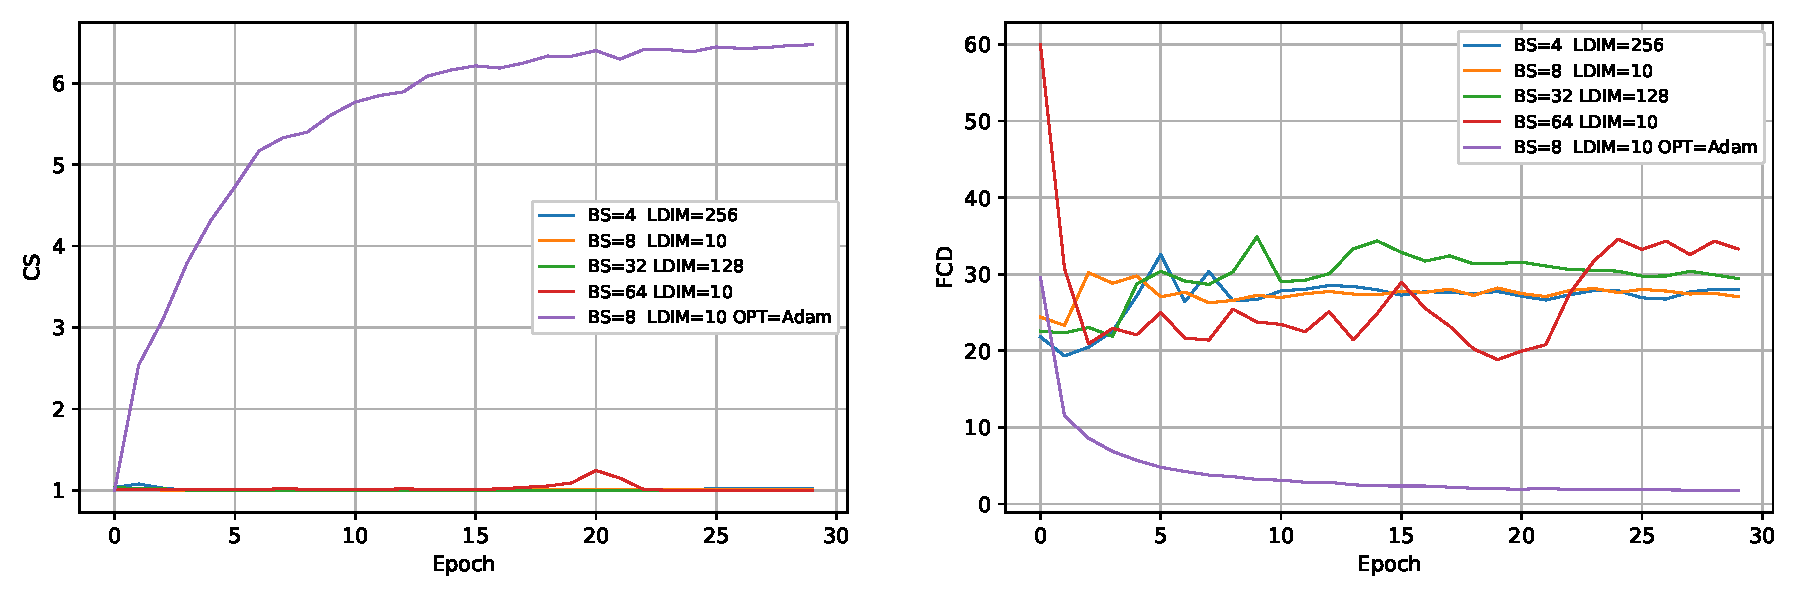
\includegraphics[width=\textwidth]{chapters/Experiments/GAN/mnist_metrics.pdf}
    \fonte{From the author (2021)}
    \label{fig:gan_mnist_metrics}
\end{figure}

Recall that for the \gls{CS}, bigger values means better, and the opposite for \gls{FCD}. Note how all choices of hyperparameters resulted in terrible values when using the \gls{SGD} with momentum optimizer, all of these cases suffered the same extreme mode collapse seen on \autoref{fig:mode_collapse_mnist}, even collapsing to the same digit. However, note how just changing to the Adam optimizer significantly increased the performance, this optimizer generally produces good results \cite{nipsGAN2017} and is one of the key components proposed in the DCGAN architecture. Given this, all following experiments will be using the Adam optimizer unless otherwise noted. \autoref{fig:gan_mnist_samples} shows samples generated from the \gls{GAN} trained with Adam.
\begin{figure}[hbt]
    \centering
    \caption{Samples when training a simple GAN on MNIST}
    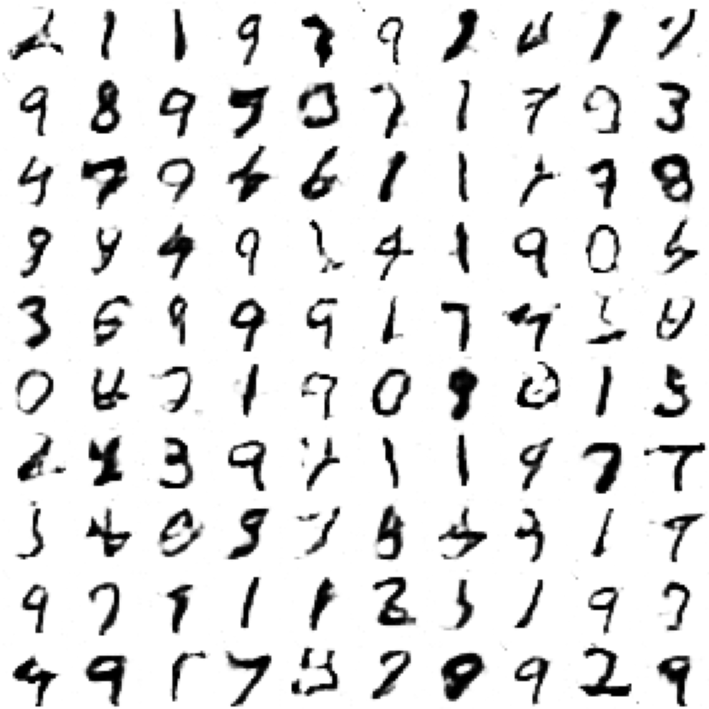
\includegraphics[width=0.4\textwidth]{chapters/Experiments/GAN/mnist_samples.png}
    \fonte{From the author (2021)}
    \label{fig:gan_mnist_samples}
\end{figure}
